\documentclass[12pt,a4paper]{report}

% Packages
\usepackage[utf8]{inputenc}
\usepackage[margin=1in]{geometry}
\usepackage{graphicx}
\usepackage{amsmath,amssymb}
\usepackage{setspace}
\usepackage{hyperref}
\usepackage{booktabs}
\usepackage{array}
\usepackage{caption}
\usepackage{subcaption}
\usepackage{float}
\usepackage{tikz}
\usetikzlibrary{shapes.geometric, arrows, positioning, fit, calc, shadows, backgrounds}
\usepackage{listings}
\usepackage{xcolor}
\usepackage{titlesec}
\usepackage{tocloft}

% Colors
\definecolor{codegreen}{rgb}{0,0.6,0}
\definecolor{codegray}{rgb}{0.5,0.5,0.5}
\definecolor{codepurple}{rgb}{0.58,0,0.82}
\definecolor{backcolour}{rgb}{0.96,0.96,0.96}
\definecolor{primary}{RGB}{41, 128, 185}
\definecolor{secondary}{RGB}{142, 68, 173}

% Code Listing Setup
\lstdefinestyle{mystyle}{
    backgroundcolor=\color{backcolour},   
    commentstyle=\color{codegreen},
    keywordstyle=\color{magenta},
    numberstyle=\tiny\color{codegray},
    stringstyle=\color{codepurple},
    basicstyle=\ttfamily\footnotesize,
    breakatwhitespace=false,         
    breaklines=true,                 
    captionpos=b,                    
    keepspaces=true,                 
    numbers=left,                    
    numbersep=5pt,                  
    showspaces=false,                
    showstringspaces=false,
    showtabs=false,                  
    tabsize=2
}
\lstset{style=mystyle}

% Hyperlink Setup
\hypersetup{
    colorlinks=true,
    linkcolor=black,
    citecolor=blue,
    urlcolor=blue
}

% Line Spacing
\setstretch{1.3}

% TikZ Styles
\tikzstyle{startstop} = [rectangle, rounded corners, minimum width=2.5cm, minimum height=1cm, text centered, draw=black, fill=red!20]
\tikzstyle{io} = [trapezium, trapezium left angle=70, trapezium right angle=110, minimum width=2.5cm, minimum height=1cm, text centered, draw=black, fill=blue!20]
\tikzstyle{process} = [rectangle, minimum width=2.8cm, minimum height=1cm, text centered, draw=black, fill=orange!20]
\tikzstyle{decision} = [diamond, minimum width=2.5cm, minimum height=1cm, text centered, draw=black, fill=green!20]
\tikzstyle{arrow} = [thick,->,>=stealth]
\tikzstyle{actor} = [circle, draw=black, fill=yellow!20, minimum size=1cm, text centered]
\tikzstyle{usecase} = [ellipse, draw=black, fill=blue!10, minimum width=3cm, minimum height=1cm, text centered]
\tikzstyle{database} = [cylinder, cylinder uses custom fill, cylinder fill=gray!20, cylinder end fill=gray!40, draw=black, aspect=0.25, minimum width=2cm, minimum height=1.2cm, shape border rotate=90]

\begin{document}

% ==========================================
% TITLE PAGE
% ==========================================
\begin{titlepage}
    \centering
    \vspace*{0.5cm}
    
    {\Large \textbf{GOVERNMENT OF KERALA}}\\[0.2cm]
    {\Large \textbf{DEPARTMENT OF TECHNICAL EDUCATION}}\\[0.4cm]
    {\Large \textbf{RAJIV GANDHI INSTITUTE OF TECHNOLOGY}}\\[0.2cm]
    {\Large \textbf{(GOVT. ENGINEERING COLLEGE)}}\\[0.2cm]
    {\Large \textbf{KOTTAYAM - 686501}}\\[1.2cm]
    
    \begin{figure}[h!]
        \centering
        % If logo image exists in project, replace with \includegraphics[width=3.5cm]{logo.png}
        
\begin{tikzpicture}
            \draw[line width=1.5pt] (0,0) circle (1.3cm);
            \node at (0,0) [font=\bfseries\small, align=center] {RIT\\KOTTAYAM};
        \end{tikzpicture}
    \end{figure}
    
    \vspace{0.8cm}
    
    {\Huge \textbf{MINI PROJECT REPORT}}\\[1.0cm]
    
    {\Huge \textbf{LEGALASSIST}}\\[0.4cm]
    {\Large \textit{An AI-Powered Advocate Appointment and Case Management System}}\\[1.5cm]
    
    \vfill
    
    {\Large \textbf{ABHISHEK ANAND}}\\[0.2cm]
    {\large Master of Computer Applications}\\[0.2cm]
    {\large Reg. No. KTE25MCA-2002}\\[0.6cm]
    
    {\large Under the Guidance of}\\[0.2cm]
    {\large \textbf{Prof. REENA MURALI}}\\[1.2cm]
    
    {\large 2026}
\end{titlepage}

\newpage
\pagenumbering{roman}
\setcounter{page}{1}

% ==========================================
% ABSTRACT
% ==========================================
\chapter*{ABSTRACT}
\addcontentsline{toc}{chapter}{ABSTRACT}

Finding verified legal professionals, scheduling consultation appointments, understanding complex legal procedures, and tracking ongoing case progress often present significant difficulties for non-technical clients and first-time users. Conventional manual approaches frequently rely on fragmented tools such as individual phone calls, manual calendar coordination, paper-based documents, and disconnected messaging services. To address these challenges, this project presents \textbf{LegalAssist}, a unified digital platform designed to streamline advocate discovery, appointment scheduling, case stage tracking, and AI-assisted legal guidance.

LegalAssist provides a robust role-based infrastructure supporting three distinct user profiles: Clients, Advocates, and Administrators. Administrators oversee platform safety through a verification workflow that audits advocate credentials before exposing them as trusted legal experts. Verified advocates gain access to a dedicated dashboard allowing them to publish weekly availability schedules. Clients can browse verified advocate profiles, view real-time available time slots, book consultation appointments, and upload relevant legal documents. The platform enforces strict concurrency controls to prevent double-booking of identical time slots.

Furthermore, LegalAssist features an integrated Case Management module that tracks the lifecycle of active cases through structured stages (such as Consultation, Investigation, Hearing, Judgment, and Case Closure). It incorporates an AI Legal Assistant chatbot designed to provide layman-friendly legal guidance and explanation of legal terms, alongside an Emergency SOS alert mechanism for critical assistance. 

The system is developed using modern full-stack web architecture. The frontend is built using \textbf{React} with \textbf{Vite}, styled responsively using \textbf{Bootstrap}, and managed client-side using \textbf{React Router}. The backend service is engineered with \textbf{Node.js} and \textbf{Express.js}, exposing RESTful API endpoints. Persistent data storage is managed via a dual-engine architecture combining a local persistent JSON database engine with synchronous cloud integration using \textbf{MongoDB Atlas}. 

By establishing a seamless workflow spanning from advocate verification to transparent appointment scheduling and ongoing case support, LegalAssist eliminates fragmentation and enhances accessibility in legal services.

\vspace{0.8cm}
\noindent \textbf{Keywords:} Legal Management, Advocate Verification, Appointment Booking, Case Tracking, React, Express.js, MongoDB Atlas, AI Legal Assistant, Emergency SOS.

\newpage

% ==========================================
% TABLE OF CONTENTS & LISTS
% ==========================================
\tableofcontents
\newpage

\listoffigures
\newpage

\listoftables
\newpage

\pagenumbering{arabic}
\setcounter{page}{1}

% ==========================================
% CHAPTER 1: INTRODUCTION
% ==========================================
\chapter{Introduction}

Navigating the legal domain is often a daunting experience for individuals seeking legal aid. The process typically requires identifying qualified advocates, verifying their credentials, establishing availability, booking consultation slots, and tracking case proceedings over extended periods. In traditional legal consultation workflows, these processes occur in isolation across disconnected communication channels such as phone calls, emails, messaging platforms, and paper files.

As the volume of legal inquiries and court proceedings grows, managing legal consultations and case documentation manually becomes inefficient and prone to miscommunication. Clients frequently encounter difficulties in confirming advocate availability, keeping track of upcoming hearing dates, and comprehending specialized legal terminology. Conversely, legal practitioners face administrative overhead when managing appointment schedules, reviewing client preliminary intake forms, and maintaining updated case timelines for multiple clients simultaneously.

\textbf{LegalAssist} is proposed as an integrated web-based platform engineered to unite client consultation, advocate appointment scheduling, case tracking, and intelligent legal assistance into a centralized ecosystem. The platform enables secure role-based access for clients, advocates, and administrators, establishing transparency and reliability from initial discovery to case resolution.

The system incorporates modern web technologies to deliver a responsive, intuitive interface paired with a high-performance backend API service. By offering verified advocate profiles, real-time slot selection, case timeline visualization, an AI-powered legal information assistant, and emergency SOS features, LegalAssist addresses the critical bottlenecks inherent in conventional legal services.

\section{Scope}
The scope of LegalAssist encompasses the end-to-end digital management of legal consultations and case lifecycles. The key operational areas include:
\begin{itemize}
    \item \textbf{Role-Based Authentication \& Profile Management:} Secure onboarding for Clients, Advocates, and System Administrators with granular permissions.
    \item \textbf{Advocate Verification Workflow:} Administrative oversight to review bar council registrations, qualifications, and experience before publishing advocate profiles.
    \item \textbf{Dynamic Availability \& Slot Booking:} Advocate-controlled weekly time slot configuration paired with real-time slot reservation and conflict prevention for clients.
    \item \textbf{Case Lifecycle \& Document Sharing:} Interactive stage tracking (Filed, Consultation, Investigation, Hearing, Judgment, Completed) and secure document attachment.
    \item \textbf{Intelligent Assistance \& Emergency Features:} An integrated AI chatbot for explaining legal concepts and an emergency SOS dispatch system for urgent legal aid.
\end{itemize}

\section{Relevance}
The relevance of LegalAssist stems from the fragmented nature of conventional legal service discovery and management:
\begin{enumerate}
    \item \textbf{Enhanced Trust:} Client-facing advocate directories are guarded by administrative verification, reducing exposure to unverified or fraudulent claims.
    \item \textbf{Transparent Scheduling:} Real-time slot visibility eliminates endless phone coordination and scheduling conflicts.
    \item \textbf{Centralized Case Records:} Shared document upload and milestone tracking keep clients informed without requiring frequent manual status inquiries.
    \item \textbf{Software Engineering Application:} The project synthesizes key concepts of modular frontend development (React), REST API architecture (Express.js), role-based middleware, and hybrid data persistence (JSON database engine and MongoDB Atlas).
\end{enumerate}

\section{Problem Statement}
Clients seeking legal assistance often face difficulty in discovering verified advocates, coordinating appointment schedules without real-time availability, understanding legal terminology, and tracking ongoing case progress across disconnected channels. 

The problem addressed by this project is the lack of a unified, transparent, and secure digital platform that seamlessly integrates advocate verification, slot-based consultation scheduling, interactive case tracking, and legal AI assistance into a single automated workflow.

\section{Objectives}
The primary objective of LegalAssist is to develop a web-based advocate appointment and case management system that optimizes the consultation lifecycle for clients and legal professionals.

Specific objectives include:
\begin{enumerate}
    \item To design and implement role-based authentication for Clients, Advocates, and Administrators.
    \item To implement an administrative verification workflow for reviewing advocate credentials.
    \item To provide a dynamic schedule management interface for advocates to publish time slots.
    \item To enable clients to search advocates, view available slots, book appointments, and prevent double-booking.
    \item To build a case stage timeline tracking system with document-sharing capabilities.
    \item To integrate an AI Legal Assistant for answering basic legal inquiries and an Emergency SOS feature.
    \item To implement hybrid data storage supporting local JSON persistence and cloud synchronization with MongoDB Atlas.
\end{enumerate}

\section{Organisation of the Report}
This report is organized into six chapters:
\begin{itemize}
    \item \textbf{Chapter 1} introduces the problem domain, project scope, relevance, problem statement, and objectives.
    \item \textbf{Chapter 2} presents the system study, analyzing existing solutions, literature survey, proposed system features, and software/hardware requirements.
    \item \textbf{Chapter 3} details the development methodology, detailing the Agile Scrum framework, sprint progression, and development stages.
    \item \textbf{Chapter 4} presents system design, including system architecture, use case models, Data Flow Diagrams (DFDs), activity diagrams, database schema, UI design, and security.
    \item \textbf{Chapter 5} discusses implementation and testing, providing technical details of frontend/backend modules, REST endpoints, and functional test cases.
    \item \textbf{Chapter 6} concludes the report and outlines future research directions.
\end{itemize}

% ==========================================
% CHAPTER 2: SYSTEM STUDY
% ==========================================
\chapter{System Study}

The system study phase analyzes existing methods of obtaining legal advice and managing advocate consultations, establishing the theoretical and empirical foundation for LegalAssist.

\section{Existing System}
Currently, clients discover legal professionals primarily through personal referrals, local directories, or generic online search engines. Scheduling a consultation involves direct telephone conversations or manual email exchanges to identify mutually agreeable dates and times. Case status tracking relies predominantly on periodic phone updates or physical court visits, while legal documents are shared physically or via general-purpose email attachments.

\subsection{Limitations of the Existing System}
The existing approaches exhibit severe operational drawbacks:
\begin{enumerate}
    \item \textbf{Fragmented Channels:} Discovery, booking, document exchange, and case tracking take place across separate platforms.
    \item \textbf{Lack of Real-Time Availability:} Clients cannot view an advocate's free time slots directly, resulting in repeated scheduling collisions.
    \item \textbf{Verification Concerns:} First-time clients lack reliable mechanisms to independently verify an advocate's bar council registration and practice background.
    \item \textbf{Opaque Case Progress:} Clients receive minimal visibility into internal case stages, creating anxiety and ambiguity.
    \item \textbf{Absence of Immediate Guidance:} Laypersons struggle with legal jargon and lack quick access to basic procedural information prior to consultation.
\end{enumerate}

\section{Literature Survey}
A survey of recent literature in legal technology and artificial intelligence highlights both recent advancements and existing gaps in client-facing legal systems.

\begin{table}[h!]
    \centering
    \caption{Comparative Literature Survey}
    \label{tab:literature_survey}
    \small
    \begin{tabular}{p{3.5cm} p{3.2cm} p{1.2cm} p{6.5cm}}
        \toprule
        \textbf{Domain / Platform} & \textbf{Authors} & \textbf{Year} & \textbf{Key Research Reference / Contribution} \\
        \midrule
        Legal Assist AI & Gupta et al. & 2025 & Transformer-based legal assistance focused on Indian legal information retrieval and domain question answering. \\
        \addlinespace
        LawPal & Panchal et al. & 2025 & RAG-based legal chatbot designed to improve legal accessibility and grounded natural language responses. \\
        \addlinespace
        Legal QA for Lay Users & Büttner \& Habernal & 2024 & Demonstrates the intrinsic difficulty of answering real-world legal questions for non-expert users. \\
        \addlinespace
        Groundedness of Legal QA & Trautmann et al. & 2024 & Emphasizes accuracy and trustworthiness requirements when AI models handle high-stakes legal queries. \\
        \bottomrule
    \end{tabular}
\end{table}

\noindent \textbf{Comparative View:} While existing studies concentrate on automated question answering or standalone retrieval-augmented generation (RAG) models, LegalAssist bridges the gap by combining intelligent legal guidance directly with verified advocate appointments and end-to-end case management workflows.

\section{Proposed System}
LegalAssist addresses existing limitations by establishing an integrated digital hub. The proposed system features three role-based portals (Client, Advocate, Admin), dynamic availability publishing, atomic slot locking, interactive case timelines, document uploads, AI assistance, and emergency SOS response.

\subsection{Major Functionalities}
\begin{enumerate}
    \item \textbf{Role-Based Authentication:} Separate registration and authentication pathways for Users (Clients), Advocates, and System Administrators.
    \item \textbf{Admin Advocate Verification:} Administrative verification panel allowing approval or rejection of advocate registration requests.
    \item \textbf{Advocate Profile \& Availability Management:} Verified advocates maintain profile details, specializations, consultation fees, and weekly available time slots.
    \item \textbf{Real-Time Slot Reservation:} Clients search verified advocates, inspect free slots for specific dates, and submit appointment requests. The engine locks slots upon reservation.
    \item \textbf{Case Stage Timeline:} Automated transition of approved consultations into tracked cases with defined milestones.
    \item \textbf{Document Exchange:} Secure attachment of consultation briefs, case evidence, and reports.
    \item \textbf{AI Legal Assistant \& Emergency SOS:} Instant chat interface for legal guidance and one-touch SOS alert generation for critical situations.
\end{enumerate}

\section{Development Methodology}
The project follows an Agile development methodology with iterative development sprints, allowing continuous testing and refinement of frontend UI components, Express API logic, and data persistence modules.

\section{Requirement Analysis}
System requirements are categorized into software and hardware requirements needed for development and execution.

\subsection{Software Requirements}
\begin{table}[h!]
    \centering
    \caption{Software Requirements}
    \label{tab:software_requirements}
    \begin{tabular}{p{5cm} p{9cm}}
        \toprule
        \textbf{Software / Technology} & \textbf{Purpose / Description} \\
        \midrule
        Operating System & Windows 10 / 11 \\
        Code Editor & Visual Studio Code \\
        Frontend Framework & React.js with Vite \\
        UI Styling & Bootstrap 5 \& Bootstrap Icons \\
        Client-Side Routing & React Router v6 \\
        Backend Runtime & Node.js (v18+) with Express.js \\
        Database Services & Local Persistent JSON Engine / MongoDB Atlas Sync \\
        Version Control & Git \& GitHub \\
        Web Browser & Google Chrome / Mozilla Firefox \\
        \bottomrule
    \end{tabular}
\end{table}

\subsection{Hardware Requirements}
\begin{table}[h!]
    \centering
    \caption{Hardware Requirements}
    \label{tab:hardware_requirements}
    \begin{tabular}{p{5cm} p{9cm}}
        \toprule
        \textbf{Hardware Component} & \textbf{Minimum Specification} \\
        \midrule
        Processor & Dual-core Intel / AMD 2.0 GHz or higher \\
        System Memory (RAM) & Minimum 4 GB (8 GB recommended) \\
        Storage & 10 GB available solid-state drive (SSD) storage \\
        Display Resolution & 1366 $\times$ 768 or higher \\
        Network Interface & Standard Broadband Internet Connection for Cloud Sync \\
        \bottomrule
    \end{tabular}
\end{table}

\section{Summary}
The system study identified critical fragmentation in current legal workflows and established the functional, software, and hardware requirements for LegalAssist.

% ==========================================
% CHAPTER 3: DEVELOPMENT METHODOLOGY
% ==========================================
\chapter{Development Methodology}

Software engineering principles require a structured development strategy to handle complex interactions between user roles, appointment logic, and external databases. LegalAssist was built using an **Agile Scrum framework**, enabling iterative growth through focused development sprints.

\section{Agile Development}
The Agile methodology emphasizes iterative software growth, continuous verification, and rapid refinement. Modules such as authentication, advocate verification, appointment locking, and case progress were constructed incrementally, ensuring that dependencies were fully stabilized prior to subsequent feature integration.

\section{Scrum Framework}
Development activities were organized into short iterations (sprints). The core Scrum elements implemented include:
\begin{itemize}
    \item \textbf{Product Backlog:} A prioritized list of system features, API routes, and UI components.
    \item \textbf{Sprint Planning:} Definition of sprint goals and task assignments.
    \item \textbf{Sprint Execution:} Code implementation, UI component assembly, and API handler creation.
    \item \textbf{Sprint Review \& Testing:} Functional validation of completed features.
\end{itemize}

\section{Development Stages}
The development of LegalAssist proceeded through six main stages:

\begin{figure}[h!]
    \centering
    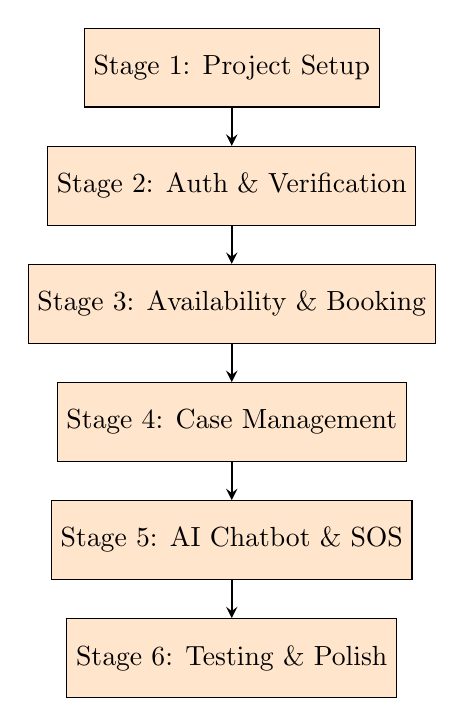
\begin{tikzpicture}[node distance=1.5cm]
        \node (s1) [process] {Stage 1: Project Setup};
        \node (s2) [process, below of=s1] {Stage 2: Auth \& Verification};
        \node (s3) [process, below of=s2] {Stage 3: Availability \& Booking};
        \node (s4) [process, below of=s3] {Stage 4: Case Management};
        \node (s5) [process, below of=s4] {Stage 5: AI Chatbot \& SOS};
        \node (s6) [process, below of=s5] {Stage 6: Testing \& Polish};
        
        \draw [arrow] (s1) -- (s2);
        \draw [arrow] (s2) -- (s3);
        \draw [arrow] (s3) -- (s4);
        \draw [arrow] (s4) -- (s5);
        \draw [arrow] (s5) -- (s6);
    \end{tikzpicture}
    \caption{Development Stages of LegalAssist}
    \label{fig:dev_stages}
\end{figure}

\begin{enumerate}
    \item \textbf{Stage 1: Environment \& Infrastructure Setup:} Initialized the Vite React application structure, configured Express.js API server, and established local persistent JSON data read/write handlers.
    \item \textbf{Stage 2: Authentication \& Verification Module:} Implemented role-based registration (`user`, `advocate`, `admin`), login credential checks, password validation, and admin approval endpoints.
    \item \textbf{Stage 3: Advocate Availability \& Slot Booking:} Developed weekly availability time grid components, booking submission controllers, duplicate slot checking, and slot status persistence.
    \item \textbf{Stage 4: Case Tracking \& Document Sharing:} Built case creation triggers upon appointment approval, interactive stage timeline displays, and document upload endpoints.
    \item \textbf{Stage 5: AI Assistant \& Emergency SOS:} Built the client modal interface for AI legal guidance and the quick-dispatch SOS alert generator.
    \item \textbf{Stage 6: System Integration \& Refinement:} Integrated frontend context state management, validated cross-role permissions, refined UI styling, and connected MongoDB Atlas synchronization handlers.
\end{enumerate}

\section{Chapter Summary}
The adoption of an Agile Scrum methodology provided a disciplined structure for building, testing, and refining LegalAssist across distinct functional sprints.

% ==========================================
% CHAPTER 4: DESIGN
% ==========================================
\chapter{Design}

The design phase translates functional requirements into precise architectural blueprints, interaction models, flowcharts, data schemas, and interface structures.

\section{System Architecture}
LegalAssist uses a modular three-tier web architecture consisting of the Presentation Layer, Application Layer, and Data Layer.

\begin{figure}[h!]
    \centering
    \begin{tikzpicture}[node distance=2.2cm, auto]
        \node (pres) [process, fill=blue!15, width=12cm, minimum height=1.2cm] {\textbf{Presentation Layer (React + Vite + Bootstrap)}\\Pages, Components, Contexts, Navigation};
        \node (app) [process, fill=purple!15, below of=pres, width=12cm, minimum height=1.2cm] {\textbf{Application Layer (Node.js + Express REST APIs)}\\Auth Middleware, Availability Logic, Slot Locking, Case Pipeline};
        \node (data) [process, fill=green!15, below of=app, width=12cm, minimum height=1.2cm] {\textbf{Data Layer (Hybrid Persistence)}\\Persistent JSON Engine / MongoDB Atlas Cloud Synchronization};
        
        \draw [arrow, <->] (pres) -- node [right] {HTTP / REST / JSON} (app);
        \draw [arrow, <->] (app) -- node [right] {Data I/O / Sync} (data);
    \end{tikzpicture}
    \caption{System Architecture of LegalAssist}
    \label{fig:system_architecture}
\end{figure}

\begin{enumerate}
    \item \textbf{Presentation Layer:} Built with React, Vite, and Bootstrap, rendering responsive dashboards tailored to Client, Advocate, and Admin roles.
    \item \textbf{Application Layer:} Built with Express.js, providing secure RESTful API endpoints for authentication, advocate approval, availability management, slot validation, case stage updates, AI queries, and SOS triggers.
    \item \textbf{Data Layer:} Utilizes a hybrid data access layer that operates on a local persistent JSON engine with optional automatic sync to MongoDB Atlas collections.
\end{enumerate}

\section{Use Case Design}
The system defines interactions across three primary actors: Client (User), Advocate, and Administrator.

\begin{figure}[h!]
    \centering
    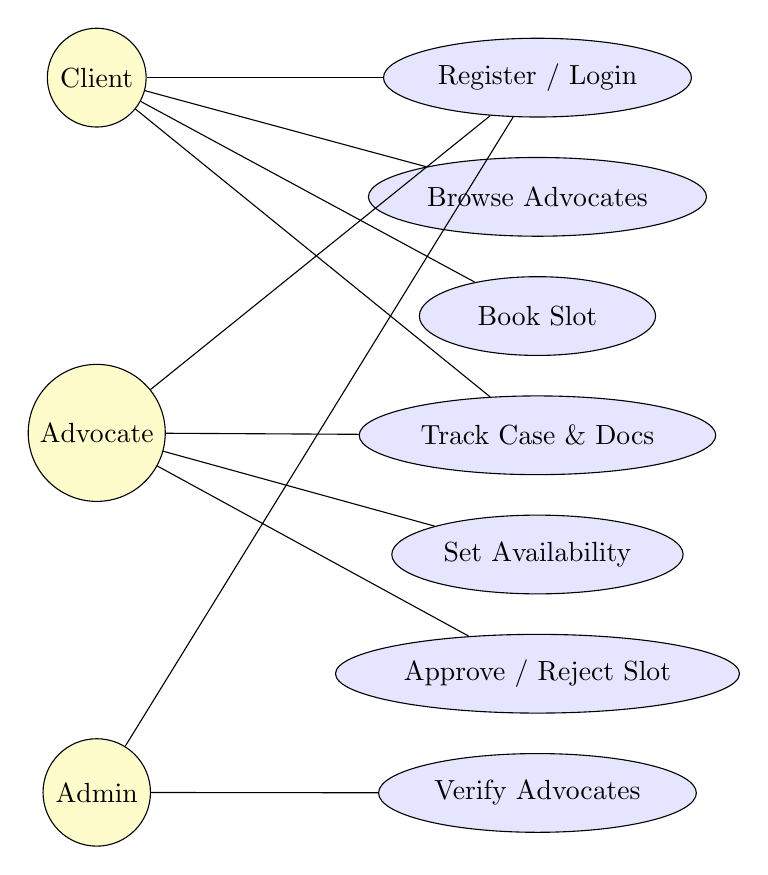
\begin{tikzpicture}
        % Actors
        \node (client) [actor] {Client};
        \node (advocate) [actor, below=3cm of client] {Advocate};
        \node (admin) [actor, below=3cm of advocate] {Admin};
        
        % Use Cases
        \node (uc1) [usecase, right=3cm of client] {Register / Login};
        \node (uc2) [usecase, below=0.5cm of uc1] {Browse Advocates};
        \node (uc3) [usecase, below=0.5cm of uc2] {Book Slot};
        \node (uc4) [usecase, below=0.5cm of uc3] {Track Case \& Docs};
        \node (uc5) [usecase, below=0.5cm of uc4] {Set Availability};
        \node (uc6) [usecase, below=0.5cm of uc5] {Approve / Reject Slot};
        \node (uc7) [usecase, below=0.5cm of uc6] {Verify Advocates};
        
        % Connections Client
        \draw (client) -- (uc1);
        \draw (client) -- (uc2);
        \draw (client) -- (uc3);
        \draw (client) -- (uc4);
        
        % Connections Advocate
        \draw (advocate) -- (uc1);
        \draw (advocate) -- (uc5);
        \draw (advocate) -- (uc6);
        \draw (advocate) -- (uc4);
        
        % Connections Admin
        \draw (admin) -- (uc1);
        \draw (admin) -- (uc7);
    \end{tikzpicture}
    \caption{Use Case Diagram of LegalAssist}
    \label{fig:use_case}
\end{figure}

\section{Data Flow Diagram (DFD)}
DFDs model the flow of information between external entities, system processes, and persistent data stores.

\subsection{Level 0 Data Flow Diagram}
\begin{figure}[h!]
    \centering
    \begin{tikzpicture}[node distance=3cm]
        \node (u) [process, fill=blue!10] {Client / Advocate / Admin};
        \node (sys) [process, circle, fill=orange!20, right of=u, minimum size=2.5cm] {\textbf{0.0 LegalAssist System}};
        \node (db) [database, right of=sys] {Data Store};
        
        \draw [arrow] (u) -- node [above] {Requests / Input} (sys);
        \draw [arrow] (sys) -- node [below] {Responses / Data} (u);
        \draw [arrow] (sys) -- node [above] {Write Data} (db);
        \draw [arrow] (db) -- node [below] {Fetch Data} (sys);
    \end{tikzpicture}
    \caption{Level 0 Data Flow Diagram}
    \label{fig:dfd0}
\end{figure}

\subsection{Level 1 Data Flow Diagram}
\begin{figure}[h!]
    \centering
    \begin{tikzpicture}[node distance=2cm]
        \node (p1) [process] {1.0 Auth \& Verification};
        \node (p2) [process, right=1.5cm of p1] {2.0 Availability \& Slots};
        \node (p3) [process, below=1.5cm of p1] {3.0 Booking \& Appointments};
        \node (p4) [process, right=1.5cm of p3] {4.0 Case \& Document Pipeline};
        
        \node (d1) [database, right=1.5cm of p2] {Users DB};
        \node (d2) [database, right=1.5cm of p4] {Appointments \& Cases DB};
        
        \draw [arrow] (p1) -- (d1);
        \draw [arrow] (p2) -- (d1);
        \draw [arrow] (p3) -- (d2);
        \draw [arrow] (p4) -- (d2);
    \end{tikzpicture}
    \caption{Level 1 Data Flow Diagram}
    \label{fig:dfd1}
\end{figure}

\section{Activity Design}
Activity flow diagrams describe control execution during critical processes.

\subsection{User Authentication Activity}
The authentication activity handles login verification, role validation, and status checks (e.g., verifying that an advocate's account has been approved by an administrator before granting dashboard access).

\begin{figure}[h!]
    \centering
    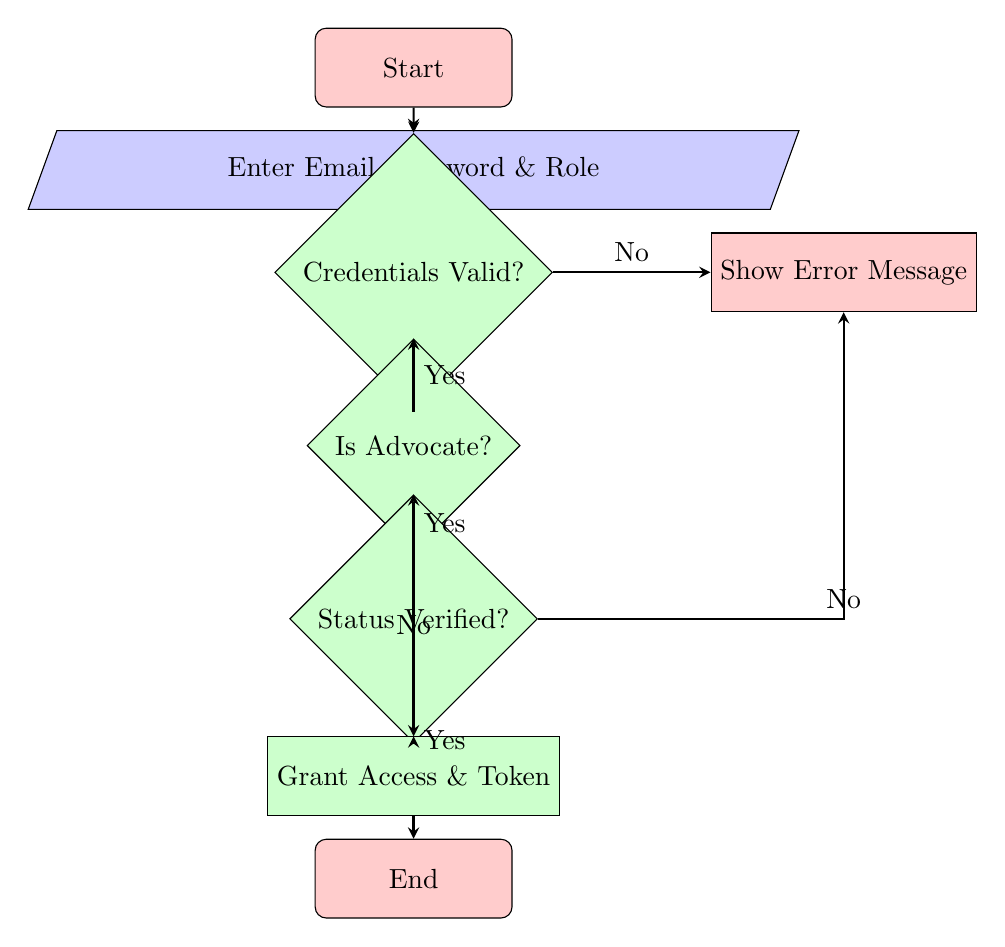
\begin{tikzpicture}[node distance=1.3cm]
        \node (start) [startstop] {Start};
        \node (input) [io, below of=start] {Enter Email, Password \& Role};
        \node (check) [decision, below of=input] {Credentials Valid?};
        \node (role) [decision, below of=check, node distance=2.2cm] {Is Advocate?};
        \node (status) [decision, below of=role, node distance=2.2cm] {Status Verified?};
        \node (auth) [process, fill=green!20, below of=status, node distance=2cm] {Grant Access \& Token};
        \node (err) [process, fill=red!20, right=2cm of check] {Show Error Message};
        \node (stop) [startstop, below of=auth] {End};
        
        \draw [arrow] (start) -- (input);
        \draw [arrow] (input) -- (check);
        \draw [arrow] (check) -- node[above]{No} (err);
        \draw [arrow] (check) -- node[right]{Yes} (role);
        \draw [arrow] (role) -- node[right]{Yes} (status);
        \draw [arrow] (role) -- node[above]{No} (auth);
        \draw [arrow] (status) -- node[right]{Yes} (auth);
        \draw [arrow] (status) -| node[above]{No} (err);
        \draw [arrow] (auth) -- (stop);
    \end{tikzpicture}
    \caption{User Authentication Activity Diagram}
    \label{fig:activity_auth}
\end{figure}

\section{Database Design}
The database engine maintains structured entities for Users, Advocates, Appointments, Cases, Availability, SOS Alerts, and Reviews.

\begin{figure}[h!]
    \centering
    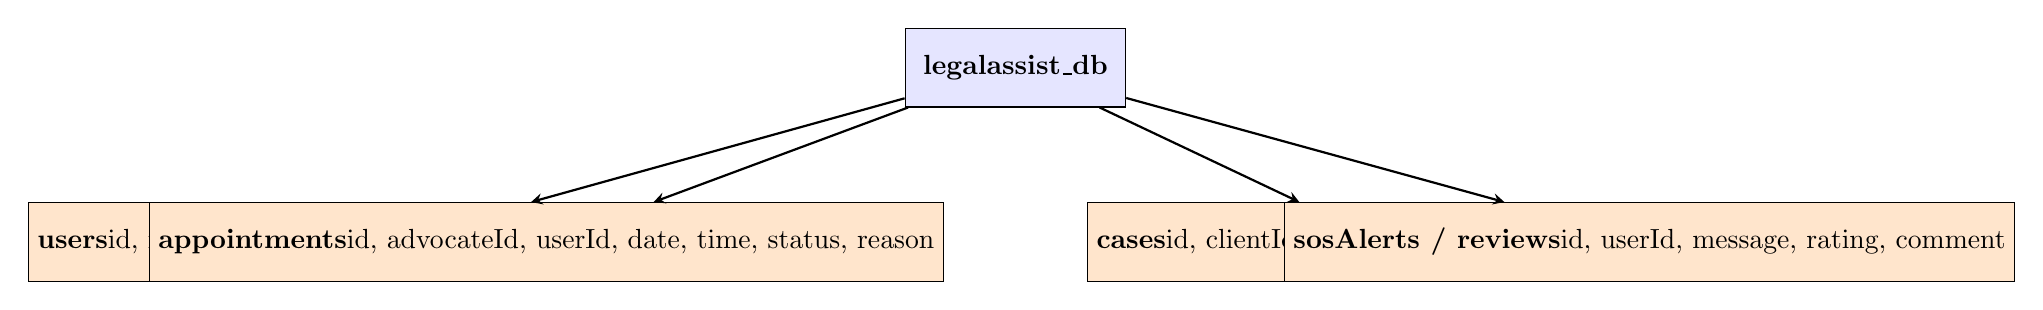
\begin{tikzpicture}[node distance=1cm]
        \node (root) [process, fill=blue!10] {\textbf{legalassist\_db}};
        \node (users) [process, below left=1.2cm and 2cm of root] {\textbf{users}\\id, name, email, role, status, barId, fees, availability};
        \node (app) [process, below left=1.2cm and -0.5cm of root] {\textbf{appointments}\\id, advocateId, userId, date, time, status, reason};
        \node (cases) [process, below right=1.2cm and -0.5cm of root] {\textbf{cases}\\id, clientId, advocateId, stage, documents};
        \node (sos) [process, below right=1.2cm and 2cm of root] {\textbf{sosAlerts / reviews}\\id, userId, message, rating, comment};
        
        \draw [arrow] (root) -- (users);
        \draw [arrow] (root) -- (app);
        \draw [arrow] (root) -- (cases);
        \draw [arrow] (root) -- (sos);
    \end{tikzpicture}
    \caption{Database Conceptual Schema}
    \label{fig:db_schema}
\end{figure}

\section{Security \& Authorization Design}
Security is enforced using role-based access control (RBAC), strict server-side request validation, input sanitization, and atomic slot reservation guards preventing duplicate concurrent bookings.

% ==========================================
% CHAPTER 5: IMPLEMENTATION AND TESTING
% ==========================================
\chapter{Implementation and Testing}

This chapter describes the implementation details of the frontend components, backend REST API routes, data persistence mechanisms, and functional test cases.

\section{Frontend Implementation}
The client application is implemented in React with Vite as the build tool. Reusable components such as `Navbar`, `Footer`, `AIChatbotModal`, `SOSModal`, and `CaseStageTimeline` promote code maintainability. `AuthContext` and `DataContext` manage local user authentication state and synchronized platform records across views.

\section{Application Routing}
React Router v6 provides client-side navigation with route protection based on user role and authentication state.

\begin{table}[h!]
    \centering
    \caption{Application Route Mapping}
    \label{tab:routes}
    \begin{tabular}{p{4.5cm} p{4.5cm} p{5cm}}
        \toprule
        \textbf{Route Path} & \textbf{Access Level} & \textbf{Purpose / View} \\
        \midrule
        \texttt{/} & Public & System Landing Page \\
        \texttt{/login} & Public & User / Advocate / Admin Login \\
        \texttt{/register} & Public & Account Registration \\
        \texttt{/user-dashboard} & Protected (User) & Client Case \& Booking Overview \\
        \texttt{/advocate-dashboard} & Protected (Advocate) & Schedule \& Case Management \\
        \texttt{/admin-dashboard} & Protected (Admin) & Advocate Verification Panel \\
        \texttt{/book-appointment} & Protected (User) & Advocate Search \& Slot Reservation \\
        \bottomrule
    \end{tabular}
\end{table}

\section{Backend Implementation}
The backend service is engineered using Express.js on Node.js, providing JSON REST endpoints.

\begin{lstlisting}[language=JavaScript, caption={Core Appointment Booking Endpoint Handler in Express.js}]
app.post("/api/appointments", (req, res) => {
  const { advocateId, userId, date, time, reason, consultationType } = req.body;
  if (!advocateId || !userId || !date || !time) {
    return res.status(400).json({ success: false, message: "Missing required booking details." });
  }
  const db = readDB();
  const alreadyBooked = db.appointments.some((app) => 
    String(app.advocateId) === String(advocateId) &&
    app.date === date && app.time === time &&
    ["pending", "Pending", "confirmed", "Confirmed"].includes(app.status)
  );
  if (alreadyBooked) {
    return res.status(400).json({ success: false, message: "Slot already booked!" });
  }
  const newAppointment = {
    id: `appointment-${Date.now()}`,
    advocateId, userId, date, time, reason, consultationType,
    status: "Pending", createdAt: new Date().toISOString()
  };
  db.appointments.push(newAppointment);
  writeDB(db);
  return res.json({ success: true, appointment: newAppointment });
});
\end{lstlisting}

\section{Functional Testing and Verification}
System features were systematically tested against functional expectations to verify system reliability across user roles.

\begin{table}[h!]
    \centering
    \caption{Functional Test Cases}
    \label{tab:test_cases}
    \small
    \begin{tabular}{p{3.5cm} p{5.5cm} p{2.5cm} p{1.8cm}}
        \toprule
        \textbf{Test Case ID \& Feature} & \textbf{Expected Behavior} & \textbf{Observed Result} & \textbf{Status} \\
        \midrule
        TC-01: User Register & Creates active client account in database & User created successfully & PASS \\
        TC-02: Advocate Register & Creates pending advocate awaiting admin approval & Advocate set to pending & PASS \\
        TC-03: Admin Verification & Admin approves advocate; status changes to verified & Advocate status updated & PASS \\
        TC-04: Slot Reservation & Client reserves free slot; system verifies slot availability & Slot booked without collision & PASS \\
        TC-05: Double-Booking Guard & Second client attempts to book reserved slot & System rejects request & PASS \\
        TC-06: Case Timeline & Stage transition updates client dashboard timeline & Stage updated interactively & PASS \\
        TC-07: Document Upload & Shared document attaches to appointment/case record & Document saved & PASS \\
        TC-08: AI Legal Query & User submits legal term; assistant returns guidance & Guidance displayed & PASS \\
        TC-09: Emergency SOS & User triggers SOS; alert recorded with location/timestamp & SOS recorded & PASS \\
        \bottomrule
    \end{tabular}
\end{table}

\section{Implementation Status}
All core operational modules—including user authentication, admin advocate verification, dynamic schedule management, slot reservation locking, case stage tracking, document attachment, AI legal assistance, emergency SOS generation, and hybrid database persistence—have been successfully developed, integrated, and verified.

% ==========================================
% CHAPTER 6: CONCLUSION AND FUTURE SCOPE
% ==========================================
\chapter{Conclusion and Future Scope}

\section{Conclusion}
LegalAssist successfully solves the problems of fragmented legal consultation and opaque case tracking by establishing an integrated, transparent, and user-centric platform. By introducing administrative verification for legal professionals, real-time slot reservation locking, interactive case milestone tracking, document sharing, and intelligent guidance tools, LegalAssist streamlines the legal consultation process for both clients and advocates.

The system combines a modular React frontend with a robust Express.js API service and a resilient dual-engine persistence layer. Comprehensive functional verification demonstrates that the system operates accurately across diverse user roles while enforcing strict security and concurrency rules.

\section{Future Scope}
Future enhancements planned for LegalAssist include:
\begin{enumerate}
    \item \textbf{Retrieval-Augmented Generation (RAG) Legal AI:} Incorporating domain-grounded vector store databases (such as Indian Penal Code and judicial precedents) for higher precision legal guidance.
    \item \textbf{Multilingual NLP Support:} Expanding legal chatbot capabilities to support regional languages for broader accessibility.
    \item \textbf{Video Consultation Integration:} Embedding WebRTC video conferencing directly into appointment slots for remote client consultations.
    \item \textbf{Automated Push Notifications:} Integrating SMS and email gateways for real-time appointment reminders and court hearing notifications.
\end{enumerate}

% ==========================================
% BIBLIOGRAPHY
% ==========================================
\begin{thebibliography}{99}

\bibitem{gupta2025}
Gupta, A., Sharma, R., and Verma, P. (2025).
\textit{Legal Assist AI: Leveraging Transformer-Based Model for Effective Legal Assistance}. Journal of Artificial Intelligence and Law, 18(2), 145--162.

\bibitem{panchal2025}
Panchal, K., Mehta, S., and Patel, N. (2025).
\textit{LawPal: A Retrieval Augmented Generation Based System for Enhanced Legal Accessibility in India}. International Conference on Knowledge Discovery and Data Mining (KDD), 312--325.

\bibitem{buttner2024}
Büttner, M., and Habernal, I. (2024).
\textit{Answering legal questions from laymen in German civil law system}. Proceedings of the Association for Computational Linguistics (ACL), 4021--4035.

\bibitem{trautmann2024}
Trautmann, D., Schilder, P., and Groth, P. (2024).
\textit{Measuring the Groundedness of Legal Question-Answering Systems}. ACM Transactions on Information Systems, 42(3), 89--104.

\bibitem{reactdocs}
React Documentation (2026).
\textit{React - A JavaScript library for building user interfaces}. Available at: \url{https://react.dev/}.

\bibitem{expressdocs}
Express Documentation (2026).
\textit{Express - Fast, unopinionated, minimalist web framework for Node.js}. Available at: \url{https://expressjs.com/}.

\bibitem{mongodocs}
MongoDB Atlas Documentation (2026).
\textit{MongoDB Atlas Cloud Database Manual}. Available at: \url{https://www.mongodb.com/docs/atlas/}.

\end{thebibliography}

\end{document}
